\documentclass[11pt, a4paper]{article}
\usepackage[a4paper, top=2.5cm, bottom=2.5cm, left=2cm, right=2cm]{geometry}
\usepackage[T1]{fontenc}
\usepackage[utf8]{inputenc}
\usepackage{tgtermes}

% --- UNIVERSAL PREAMBLE BLOCK ---
\usepackage[english, provide=*]{babel}
\babelprovide[import, onchar=ids fonts]{english}

\usepackage{amsmath}
\usepackage{amssymb}
\usepackage{amsfonts}
\usepackage{amsthm}
\usepackage{booktabs}
\usepackage{microtype}
\usepackage{xcolor}
\usepackage{graphicx}
\graphicspath{{results/}}
\usepackage{enumitem}

\setlist[itemize]{label=-}

% Theorem Environments

\newtheorem{theorem}{Theorem}[section]

\newtheorem{lemma}[theorem]{Lemma}

\newtheorem{proposition}[theorem]{Proposition}

\newtheorem{definition}[theorem]{Definition}

\newtheorem{remark}[theorem]{Remark}

\newtheorem{corollary}[theorem]{Corollary}

% Custom Command Definitions

\newcommand{\hilb}{\mathcal{H}}

\newcommand{\dd}{\mathrm{d}}

\newcommand{\ee}{\mathrm{e}}

\newcommand{\ii}{\mathrm{i}}

\newcommand{\bra}[1]{\langle #1 |}

\newcommand{\ket}[1]{| #1 \rangle}

\newcommand{\bracket}[2]{\langle #1 | #2 \rangle}

\newcommand{\opvalue}[3]{\langle #1 | #2 | #3 \rangle}

\newcommand{\norm}[1]{\| #1 \|}

\newcommand{\Tr}{\operatorname{Tr}}

\newcommand{\Herm}{\operatorname{Herm}}

\newcommand{\spec}{\operatorname{spec}}

% Generated by summarize_section7_results.py; do not edit.
\providecommand{\SectionSevenResultSchema}{4}
\providecommand{\SectionSevenInstanceCount}{40}
\providecommand{\SectionSevenCsvSha}{\texttt{b73a094cf3b5c612d6b1b488311a4da6c1f9c7a515cd23648a9939cb52c8c901}}
\providecommand{\SectionSevenGraphArchiveSha}{\texttt{0325f5fcc2ea08ef2e3719af0d5210410a8f886abac26c005f0f18f0361bc4d8}}
\providecommand{\SectionSevenWeightRows}{%
10 & 26.567446 & 26.567446 & 26.567446 & 18/20 \\%
12 & 38.036511 & 38.036511 & 38.036511 & 20/20 \\%
}
\providecommand{\SectionSevenGapDiameterRows}{%
10 & 22.32 & 36.57 & 1.64 \\%
12 & 30.52 & 50.04 & 1.64 \\%
}
\providecommand{\SectionSevenGlobalConditionalRows}{%
10 & 20/20 & $2.117\times 10^{-2}$ & $4.849\times 10^{-5}$ & $4.630\times 10^{-2}$ \\%
12 & 19/20 & $1.736\times 10^{-2}$ & 0 & $4.802\times 10^{-2}$ \\%
}
\providecommand{\SectionSevenSolveCountRows}{%
10 & $148.0\,/\,147.65 \pm 13.21$ & $97.0\,/\,124.30 \pm 79.59$ & $14.06\% \pm 57.76\%$ & $-132.14\%$ & $32.80\%$ & $69.64\%$ \\%
12 & $201.5\,/\,201.60 \pm 15.80$ & $170.5\,/\,330.85 \pm 506.68$ & $-74.11\% \pm 286.68\%$ & $-1102.79\%$ & $14.35\%$ & $70.50\%$ \\%
}
\providecommand{\SectionSevenUnresolvedRows}{%
10 & $20/20$ & 0.00 & 0 & 0 \\%
12 & $19/20$ & 0.05 & $5.000\times 10^{-5}$ & $1.000\times 10^{-3}$ \\%
}
\providecommand{\SectionSevenCoverageRows}{%
10 & 0.0756 & 0.2311 & 0.1341 \\%
12 & 0.0550 & 0.1619 & 0.0983 \\%
}


\usepackage[colorlinks=true, linkcolor=blue, citecolor=magenta, urlcolor=teal]{hyperref}

\title{\textbf{Shift-Invariant Gap Continuation and Selected Replayable Level-3 Anchors}}

\author{
  \textbf{Tiago Verissimo}\\
  \small \textit{School of Mathematics, Statistics and Physics at Newcastle University} \\
}
\date{}

\setcounter{secnumdepth}{2}

\begin{document}

\maketitle

\begin{abstract}
We study lower-bound propagation for the instantaneous spectral gap of affine Hamiltonian paths. For $D=H_P-H_I$, Weyl's inequalities give the shift-invariant constant
\begin{equation*}
K_{\mathrm{gap}}=\lambda_{\max}(D)-\lambda_{\min}(D)
=2\min_{c\in\mathbb R}\norm{D-cI}_2.
\end{equation*}
For archived binary64 Max-Cut weights interpreted as exact dyadic rationals, the schema-4 runs use an outward-rounded direct bound $K_{\mathrm{gap,cert}}\ge W_{\mathrm{exact}}+\Lambda_I$, never the older $2(W+n_v)$ comparison. The continuation sweep uses ordinary adaptive steps and an exponential mark-and-probe rule after floor triggers; every interval is classified from the actual-length bound $B_k$. Its continuous-path outputs remain Level~2 because the sparse anchor indexing is conditional. Separately, replayable exact records and an independent comparison-matrix and interlacing checker verify four selected exact-dyadic seed-0 anchors at Level~3, without upgrading either continuous sweep. Perron--Frobenius structure already supplies interior ground-state uniqueness for the retained benchmark class, so the experiments assess quantitative lower bounds and workload rather than discover positivity. Positive-semidefinite monotonicity remains only a supplementary componentwise comparison.
\end{abstract}

\section{Introduction and Motivation}
Adiabatic quantum computing (AQC) evolves from a driver Hamiltonian $H_I$ toward a problem Hamiltonian $H_P$, commonly through the affine path introduced in \cite{farhi2000quantumcomputationadiabaticevolution},
\begin{equation}
H(s)=(1-s)H_I+sH_P, \qquad s\in[0,1].
\end{equation}
Writing its two lowest ordered eigenvalues as $E_0(s)$ and $E_1(s)$, the instantaneous gap and its minimum are
\begin{equation}
\Delta(s)=E_1(s)-E_0(s),
\qquad
\Delta_{\min}=\min_{s\in[0,1]}\Delta(s).
\end{equation}
The frequently quoted condition
\begin{equation}
T \gg \frac{\max_s \left| \opvalue{\psi_1(s)}{\frac{\dd H(s)}{\dd s}}{\psi_0(s)} \right|}{\Delta_{\min}^2}
\end{equation}
is a useful heuristic scaling relation, not a general adiabatic theorem. Rigorous formulations impose additional smoothness and derivative conditions. Small gaps, including those associated with first-order quantum phase transitions, can make adiabatic evolution costly \cite{smelyanskiy2002dynamicsquantumadiabaticevolution,PhysRevResearch.5.043236}; alternative paths and catalysts are therefore widely studied \cite{PhysRevResearch.5.043236,hnzj-j7kt,farhi2000quantumcomputationadiabaticevolution}.

This paper asks a narrower verification question: how can a lower bound known at finitely many parameter values be propagated between them? For $D=H_P-H_I$, the scalar part of $D$ shifts all energies equally and cannot change a gap. We therefore use
\begin{equation}
K_{\mathrm{gap}}=\lambda_{\max}(D)-\lambda_{\min}(D)
\end{equation}
rather than taking $2\norm{D}_2$ as the primary bound. In the archived benchmark, binary64 weights are exact dyadic inputs, $W_{\mathrm{exact}}$ is their exact rational sum, and $K_{\mathrm{gap,cert}}$ is rounded upward so that
\begin{equation}
K_{\mathrm{gap,cert}}\ge W_{\mathrm{exact}}+\Lambda_I\ge K_{\mathrm{gap}}.
\end{equation}
Ordinary adaptive steps use $\eta\Delta_{+,\mathrm{lo}}/K_{\mathrm{gap,cert}}$. A floor trigger instead marks the interval, advances by an exponentially growing capped probe, and resolves it only when the bound computed from the actual clipped length is positive.

All matrix inequalities used here are classical. The methodological contribution is their assembly into an explicit continuation and auditable schema-4 record format, together with a finite-size workload assessment. The continuous sweeps use conditionally indexed floating-point anchors and remain Level~2. Four selected exact-dyadic anchors have replayable records and independent Level-3 checks at those points only. The retained Max-Cut paths also have Perron--Frobenius ground-state uniqueness in the interior and are filtered for endpoint nondegeneracy, so the aggregate experiment measures the strength and cost of the lower-bound construction rather than whether the mathematical path is open. The PSD results are supplementary and do not drive the algorithm.

\section{Related Work and Scope}
This paper positions itself at the intersection of classical matrix analysis and the physical engineering of adiabatic pathways. The literature driving this study can be categorized into three major streams:

\subsection{Classical Spectral Stability and Subspace Rotations}
The static behavior of eigenvalues under additive perturbations is governed by the regular perturbation theory of Kato \cite{Kato1966} and the spectral variation metrics surveyed by Bhatia \cite{Bhatia2007}. While Weyl's inequalities provide worst-case estimates on individual eigenvalues, they ignore eigenvector geometry. To address how state vectors track these moving energy levels, the numerical linear algebra community developed eigenspace stability bounds, most notably the Davis-Kahan $\sin\theta$ theorem \cite{DavisKahan1970} and its modern $\ell_\infty$ and small-gap refinements \cite{Fan2018, TranVu2022}. These eigenspace stability bounds are complementary to our eigenvalue-only certificates and could support future extensions to state-tracking certification.

\subsection{Rigorous Adiabatic Theorems and Local Scheduling}
The ``folk'' condition $T\propto\Delta^{-2}$ is generally insufficient by itself to guarantee high-fidelity state tracking. Rigorous adiabatic theorems, including those of Jansen, Ruskai, and Seiler \cite{JRS2007}, give bounds involving path derivatives and the gap. Local schedules such as the Roland--Cerf rule $\dd s/\dd t\propto\Delta^2(s)$ \cite{RolandCerf2002} slow the evolution near small gaps. Valid interval gap lower bounds could be used as inputs to such analyses, but this paper does not derive a runtime guarantee.

Werner et al.\ \cite{PhysRevResearch.5.043236} estimate the location $s^*$ of a minimum gap from graph-theoretic information. Our complementary objective is to propagate supplied lower bounds and identify intervals that the chosen continuation data do or do not resolve.

\subsection{Constraints, Catalysts, and the Scope of PSD Comparisons}
QUBO penalty constructions are surveyed by Lucas \cite{Lucas2014}, while stoquastic and non-stoquastic catalysts have been studied as path modifications near difficult transitions \cite{SekiNishimori2012, Albash2019, Crosson2020designing}. Spectral gap amplification in the sense of Somma and Boixo \cite{SommaBoixo2013} is a separate construction with additional structure. The elementary PSD monotonicity statements below say only that adding a PSD term cannot lower an ordered eigenvalue. Because the ground and excited energies may rise by different amounts---or by the same scalar shift---this observation neither predicts catalyst performance nor constitutes a catalyst-design principle.

\subsection{Verified Eigensolvers and Eigenvalue Enclosures}
Verified numerical linear algebra can provide rigorous indexed eigenvalue enclosures using interval arithmetic, variational bounds, or verified inertia calculations \cite{Rump2010Acta,Temple1928,Kato1949,Lehmann1950}. Residual norms from an ordinary floating-point sparse solve provide only spectral-existence information near Ritz values and do not identify eigenvalue indices. The selected replayable exact anchors below instead combine an exact Rayleigh upper bound with a comparison-matrix lower bound for a principal submatrix and Cauchy interlacing. Their exact-dyadic specifications and no-tolerance checker make the pointwise results independently reproducible; this is a classical finite-dimensional route to indexed verification, not a claim that the floating-point continuation has become fully verified.

The individual matrix inequalities used here are classical. The paper's scope is to specialize the shift-invariant Weyl bound to affine AQC gaps, make the continuation and mark-and-probe bookkeeping explicit, and demonstrate both a conditional Level-2 sweep and a small set of separately verified, replayable Level-3 anchors.

\section{Contributions}

For the affine path $H(s)=H_I+sD$, $D=H_P-H_I$, the paper makes the following limited methodological contributions.
\begin{enumerate}
    \item \textbf{Shift-invariant gap propagation.} Weyl's inequalities give
    \begin{equation}
    |\Delta(t)-\Delta(s)|\le K_{\mathrm{gap}}|t-s|,
    \qquad
    K_{\mathrm{gap}}=\lambda_{\max}(D)-\lambda_{\min}(D)
    =2\min_{c\in\mathbb R}\norm{D-cI}_2.
    \end{equation}
    The conventional $2\norm{D}_2$ estimate is retained only for comparison.

    \item \textbf{Continuation and mark-and-probe bookkeeping.} The schema-4 sweep uses the direct $K_{\mathrm{gap,cert}}$, records proposed, floor-overridden, probe-planned, and actual clipped lengths, and classifies every interval by $B_k>0$. Exponential probing avoids repeated microscopic floor steps without silently claiming the skipped region. A positive floor still gives unconditional and refined termination bounds, including the case $K_{\mathrm{gap,cert}}=0$.

    \item \textbf{Exact indexed anchor verification.} A comparison-matrix theorem combines scaled diagonal dominance, a quadratic-form comparison, Cauchy interlacing, and an exact Rayleigh quotient. Replayable exact rational records and an independent checker apply this result to four selected seed-0 anchors. These pointwise Level-3 results do not verify either continuous sweep.

    \item \textbf{Complementary PSD comparisons.} Componentwise Weyl monotonicity and Rayleigh--Ritz yield elementary energy and gap lower bounds under PSD hypotheses. They do not order catalyzed gaps and are not catalyst-design results.
\end{enumerate}

The aggregate tables are imported from the generated schema-\SectionSevenResultSchema{} summary rather than transcribed by hand. Their continuous-path lower bounds remain conditional on floating-point eigenvalue indexing.

\section{Mathematical Preliminaries}

This section fixes the notation used throughout the paper. The basic definitions are standard in quantum information theory; for further background, see \cite{Nielsen_Chuang_2010} and \cite{Watrous_2018}. Let $\hilb \cong \mathbb{C}^{2^N}$ denote the finite-dimensional Hilbert space representing $N$ qubits.
\begin{definition}[Hermitian Operators]
An operator $H: \hilb \to \hilb$ is self-adjoint (Hermitian) if $H = H^\dagger$. We denote the set of $d \times d$ Hermitian matrices as $\Herm(d)$, where $d = 2^N$.
\end{definition}

By the spectral theorem, as presented in \cite{Watrous_2018}, any $H \in \Herm(d)$ possesses a complete orthonormal eigenbasis with real eigenvalues. Throughout the paper, generic matrix eigenvalues are indexed from $1$ to $d$ and ordered as
\begin{equation}
\lambda_1(H)\le \lambda_2(H)\le \cdots \le \lambda_d(H),
\qquad
\spec(H)=\{\lambda_1(H),\lambda_2(H),\dots,\lambda_d(H)\}.
\end{equation}

\begin{definition}[Spectral Norm]
The spectral norm (or operator norm) of an operator $A$ on $\hilb$, denoted $
\norm{A}_2$, is its largest singular value:
\begin{equation}
\norm{A}_2 \equiv \sup_{\ket{\phi} \neq 0} \frac{\norm{A\ket{\phi}}}{\norm{\ket{\phi}}}.
\end{equation}
\end{definition}

\begin{remark}
For Hermitian $A$, the spectral theorem immediately gives
\begin{equation}
\norm{A}_2=\max_{1\le j\le d}|\lambda_j(A)|
=\max\{|\lambda_1(A)|,|\lambda_d(A)|\}.
\end{equation}
\end{remark}

The underlying mathematical machinery driving both variational ceilings and Weyl-type stability bounds is the Courant--Fischer minimax theorem \cite{Bhatia2007}. For any self-adjoint operator $H \in \Herm(d)$ with ordered eigenvalues $\lambda_1 \le \lambda_2 \le \dots \le \lambda_d$, the theorem provides a variational characterization of the entire spectrum:

\begin{equation}
\label{eq:courant-fischer}
\lambda_k(H) = \min_{\dim V = k} \, \max_{|f\rangle \in V \setminus \{0\}} \frac{\langle f | H | f \rangle}{\langle f | f \rangle} = \max_{\dim W = d-k+1} \, \min_{|f\rangle \in W \setminus \{0\}} \frac{\langle f | H | f \rangle}{\langle f | f \rangle}
\end{equation}

This variational foundation also underpins modern Quantum Subspace Diagonalization (QSD) and quantum Krylov methods \cite{Parrish2019, Stair2020}.

In AQC, the interpolating Hamiltonian $H(s)$ is a continuous curve in $\Herm(d)$. To emphasize the ground state, instantaneous energy levels are indexed from $0$ to $d-1$:
\begin{equation}
H(s)\ket{\psi_k(s)}=E_k(s)\ket{\psi_k(s)},
\qquad
E_0(s)\le E_1(s)\le \cdots \le E_{d-1}(s).
\end{equation}
The gap function is $\Delta(s)=E_1(s)-E_0(s)$. Thus $E_k(s)$ corresponds to $\lambda_{k+1}(H(s))$ under the generic matrix-indexing convention.

\section{Shift-Invariant Weyl Gap Bounds and PSD Comparisons}

Weyl's inequalities control ordered eigenvalues under Hermitian perturbations. Applied directly to the difference of two energy levels, they retain only the spectral width of the perturbation and discard its gap-irrelevant scalar part.

\subsection{Weyl's Perturbation Theorem}
\begin{theorem}[Weyl's Inequality]
\label{thm:weyl}
Let $A, B \in \Herm(d)$ be two Hermitian matrices, and let $C = A + B$. Let the eigenvalues of $A, B,$ and $C$ be sorted in non-decreasing order:
\begin{equation}
\lambda_k(A), \quad \lambda_k(B), \quad \lambda_k(C) \quad \text{for } k=1,\dots,d
\end{equation}
Then, for every $k \in \{1, \dots, d\}$, the following inequality holds:
\begin{equation}
\lambda_k(A) + \lambda_1(B) \le \lambda_k(A + B) \le \lambda_k(A) + \lambda_d(B)
\end{equation}
\end{theorem}

\begin{proof}
See Bhatia \cite{Bhatia2007} for a proof of the standard Weyl inequalities using variational eigenvalue characterizations.
\end{proof}

An immediate and powerful corollary of Weyl's Inequality relates the spectral norm of the perturbation to the maximum possible shift in any eigenvalue.

\begin{corollary}[Eigenvalue Stability]
\label{cor:eigenvalue-stability}
Let $A, B \in \Herm(d)$. Then
\begin{equation}
|\lambda_k(A + B) - \lambda_k(A)| \le
\norm{B}_2, \quad \forall k \in \{1, \dots, d\}
\end{equation}
\end{corollary}
\begin{proof}
For Hermitian $B$, $-\norm{B}_2\le\lambda_1(B)\le\lambda_d(B)\le\norm{B}_2$. Substitution in Theorem~\ref{thm:weyl} gives the result.
\end{proof}

\begin{corollary}[Positive-Semidefinite Monotonicity]
\label{cor:psd-monotonicity}
Let $A,B\in\Herm(d)$ and suppose $B\ge0$. Then
\begin{equation}
\lambda_k(A)\le \lambda_k(A+B),\qquad k=1,\ldots,d.
\end{equation}
\end{corollary}

\begin{proof}
  Since $B\ge 0$, its smallest eigenvalue satisfies $\lambda_1(B)\ge 0$. The result follows by applying Theorem~\ref{thm:weyl}.
\end{proof}


\subsection{Shift-Invariant Lipschitz Bound for an Affine AQC Gap}

\begin{theorem}[Shift-Invariant Lipschitz Bound for the Adiabatic Gap]
\label{thm:lipschitz-gap}
Let
\begin{equation}
H(s)=H_I+sD=(1-s)H_I+sH_P,
\qquad D:=H_P-H_I,
\qquad s\in[0,1],
\end{equation}
with $H_I,H_P\in\Herm(d)$. Let $E_0(s)\le\cdots\le E_{d-1}(s)$ be the ordered eigenvalues and $\Delta(s)=E_1(s)-E_0(s)$. Define
\begin{equation}
\label{eq:gap-lipschitz-constant}
K_{\mathrm{gap}}:=\lambda_{\max}(D)-\lambda_{\min}(D).
\end{equation}
Then, for all $s,t\in[0,1]$,
\begin{equation}
\label{eq:lipschitz-gap}
|\Delta(t)-\Delta(s)|\le K_{\mathrm{gap}}|t-s|.
\end{equation}
Moreover,
\begin{equation}
\label{eq:shift-invariant-norm}
K_{\mathrm{gap}}
=2\min_{c\in\mathbb R}\norm{D-cI}_2,
\end{equation}
and the minimum is attained at
\begin{equation}
c_* = \frac{\lambda_{\max}(D)+\lambda_{\min}(D)}{2}.
\end{equation}
If $K_{\mathrm{gap}}=0$, then $D=c_*I$ and $\Delta(s)$ is constant on $[0,1]$.
\end{theorem}

\begin{proof}
Set $m=\lambda_{\min}(D)$ and $M=\lambda_{\max}(D)$. Suppose first that $t\ge s$ and write $\alpha=t-s$. Since $H(t)=H(s)+\alpha D$, Theorem~\ref{thm:weyl} gives, for every $j$,
\begin{equation}
E_j(s)+\alpha m\le E_j(t)\le E_j(s)+\alpha M.
\end{equation}
Using the lower estimate for $E_1(t)$ and the upper estimate for $E_0(t)$, and then reversing those choices, yields
\begin{equation}
\Delta(s)-\alpha(M-m)
\le\Delta(t)\le
\Delta(s)+\alpha(M-m).
\end{equation}
Thus Eq.~\eqref{eq:lipschitz-gap} holds when $t\ge s$; interchanging $s$ and $t$ handles the other order.

For any $c\in\mathbb R$, the extreme eigenvalues of $D-cI$ are $m-c$ and $M-c$, so
\begin{equation}
\norm{D-cI}_2=\max\{|m-c|,|M-c|\}.
\end{equation}
The triangle inequality implies
\begin{equation}
M-m\le |M-c|+|m-c|\le2\norm{D-cI}_2.
\end{equation}
At $c=c_*=(M+m)/2$, both endpoint distances equal $(M-m)/2$, proving Eq.~\eqref{eq:shift-invariant-norm}. Finally, $K_{\mathrm{gap}}=0$ means $M=m$; the spectral theorem then gives $D=mI$, which changes only the common energy origin and leaves every gap constant.
\end{proof}

\begin{corollary}[Conventional Spectral-Norm Comparison]
\label{cor:conventional-gap-bound}
Under the hypotheses of Theorem~\ref{thm:lipschitz-gap},
\begin{equation}
K_{\mathrm{gap}}\le2\norm{D}_2,
\qquad
|\Delta(t)-\Delta(s)|\le2\norm{D}_2|t-s|.
\end{equation}
\end{corollary}
\begin{proof}
Choose $c=0$ in Eq.~\eqref{eq:shift-invariant-norm}.
\end{proof}

\begin{remark}[Propagation from one anchor]
Let $\delta_0>0$ be a valid lower bound on $\Delta(s_0)$ and let $K_{\mathrm{gap,cert}}\ge K_{\mathrm{gap}}$. Then
\begin{equation}
\Delta(s)\ge\delta_0-K_{\mathrm{gap,cert}}|s-s_0|.
\end{equation}
If $K_{\mathrm{gap,cert}}>0$, the right-hand side is positive for $|s-s_0|<\delta_0/K_{\mathrm{gap,cert}}$. If $K_{\mathrm{gap,cert}}=0$, the gap is constant and the positive anchor bound propagates across the entire path.
\end{remark}

\subsection{Exact Indexed Anchor Verification by a Comparison Matrix}

\begin{theorem}[Exact Indexed Anchor Bound from a Positive Witness]
\label{thm:exact-indexed-anchor}
Let $H\in\mathbb R^{d\times d}$ be real symmetric with ordered eigenvalues
\begin{equation}
E_0(H)\le E_1(H)\le\cdots\le E_{d-1}(H).
\end{equation}
Delete coordinate $p$ to form the principal submatrix $A=H^{(p)}\in\mathbb R^{(d-1)\times(d-1)}$, and define its comparison matrix $M$ by
\begin{equation}
M_{ii}=A_{ii},
\qquad
M_{ij}=-|A_{ij}|\quad(i\ne j).
\end{equation}
For any vector $x\in\mathbb R^{d-1}$ with $x_i>0$ for every $i$, set
\begin{equation}
\ell:=\min_i\frac{(Mx)_i}{x_i}.
\end{equation}
Then
\begin{equation}
E_1(H)\ge\lambda_{\min}(A)\ge\ell.
\end{equation}
Moreover, for any nonzero $q\in\mathbb R^d$, the exact Rayleigh quotient
\begin{equation}
U_0:=\frac{q^{\mathsf T}Hq}{q^{\mathsf T}q}
\end{equation}
satisfies $E_0(H)\le U_0$, and hence
\begin{equation}
\label{eq:exact-anchor-gap}
\Delta(H)=E_1(H)-E_0(H)\ge\ell-U_0.
\end{equation}
In particular, $\ell-U_0>0$ is an exact indexed gap certificate at that anchor.
\end{theorem}

\begin{proof}
By definition of $\ell$, $(M-\ell I)x\ge0$ componentwise. Let $R=\operatorname{diag}(x_1,\ldots,x_{d-1})$. The symmetric matrix
\begin{equation}
S:=R(M-\ell I)R
\end{equation}
has nonpositive off-diagonal entries. For every row $i$, the inequality $((M-\ell I)x)_i\ge0$ gives
\begin{equation}
S_{ii}=x_i^2(M_{ii}-\ell)
\ge x_i\sum_{j\ne i}|M_{ij}|x_j
=\sum_{j\ne i}|S_{ij}|.
\end{equation}
Thus $S$ is symmetric diagonally dominant with nonnegative diagonal and is positive-semidefinite. Since $R$ is invertible, congruence implies $M-\ell I\ge0$.

For arbitrary $y\in\mathbb R^{d-1}$, put $z_i=|y_i|$. The definition of $M$ and the preceding bound give
\begin{align}
y^{\mathsf T}Ay
&\ge \sum_i A_{ii}y_i^2-2\sum_{i<j}|A_{ij}|\,|y_i|\,|y_j|\\
&=z^{\mathsf T}Mz
\ge\ell\norm{z}_2^2
=\ell\norm{y}_2^2.
\end{align}
Therefore $\lambda_{\min}(A)\ge\ell$. Cauchy interlacing for a principal submatrix gives
\begin{equation}
E_0(H)\le\lambda_{\min}(A)\le E_1(H),
\end{equation}
so $E_1(H)\ge\ell$. Finally, Rayleigh--Ritz gives $E_0(H)\le U_0$ for every nonzero $q$, and subtraction proves Eq.~\eqref{eq:exact-anchor-gap}.
\end{proof}

\begin{remark}
The theorem is a classical comparison-and-interlacing certificate. Its force in an implementation comes from checking the input matrix, positive witness, componentwise inequalities, and Rayleigh quotient in exact arithmetic rather than from a floating-point tolerance.
\end{remark}

\subsection{Complementary Positive-Semidefinite Bounds}

\begin{proposition}[Componentwise Floors and a Gap Lower Bound]
\label{prop:componentwise-floors}
Assume that the initial and problem Hamiltonians are positive-semidefinite,
\begin{equation}
H_I\ge 0,
\qquad
H_P\ge 0,
\end{equation}
and consider the affine adiabatic path
\begin{equation}
H(s)=(1-s)H_I+sH_P,
\qquad s\in[0,1].
\end{equation}
Let the eigenvalues of $H(s)$ be written as
\begin{equation}
E_0(s)\le E_1(s)\le \cdots \le E_{d-1}(s),
\end{equation}
and write the eigenvalues of $H_I$ and $H_P$ in the same non-decreasing order. Then, for every $k=0,\dots,d-1$,
\begin{equation}
\label{eq:componentwise-floor}
E_k(s)
\ge
\max\{(1-s)E_k(H_I),\,sE_k(H_P)\}.
\end{equation}
Moreover, if $\ket{\psi_I}$ is a normalized ground state of $H_I$, then the first spectral gap satisfies the lower bound
\begin{equation}
\label{eq:psd-gap-bound}
\Delta(s)
\ge
\max\{(1-s)E_1(H_I),\,sE_1(H_P)\}
-(1-s)E_0(H_I)-s\opvalue{\psi_I}{H_P}{\psi_I}.
\end{equation}
\end{proposition}

\begin{proof}
Fix $s\in[0,1]$. Since $H_P\ge 0$, the operator $sH_P$ is positive-semidefinite. We may therefore apply the positive-semidefinite monotonicity corollary to
\begin{equation}
A=(1-s)H_I,
\qquad
B=sH_P.
\end{equation}
This gives, for every eigenvalue index $k$,
\begin{equation}
E_k(s)=E_k(A+B)
\ge E_k(A).
\end{equation}
Because $1-s\ge 0$, scaling the Hamiltonian $H_I$ by $1-s$ scales all of its eigenvalues by $1-s$. Hence
\begin{equation}
E_k(s)
\ge
(1-s)E_k(H_I).
\end{equation}
Similarly, since $(1-s)H_I$ is positive-semidefinite, we can instead write
\begin{equation}
A=sH_P,
\qquad
B=(1-s)H_I.
\end{equation}
Applying the same corollary gives
\begin{equation}
E_k(s)=E_k(A+B)
\ge E_k(A)=sE_k(H_P).
\end{equation}
Combining the two lower bounds yields
\begin{equation}
E_k(s)
\ge
\max\{(1-s)E_k(H_I),\,sE_k(H_P)\}.
\end{equation}
This proves the componentwise eigenvalue floor.

To obtain a lower bound on the spectral gap, we combine a lower bound on $E_1(s)$ with an upper bound on $E_0(s)$. Taking $k=1$ in the componentwise estimate gives
\begin{equation}
E_1(s)
\ge
\max\{(1-s)E_1(H_I),\,sE_1(H_P)\}.
\end{equation}
On the other hand, the variational principle gives, for any normalized trial state $\ket{\psi}$,
\begin{equation}
E_0(s)\le \opvalue{\psi}{H(s)}{\psi}.
\end{equation}
Choosing $\ket{\psi}=\ket{\psi_I}$, where $\ket{\psi_I}$ is a ground state of $H_I$, gives
\begin{align}
E_0(s)
&\le \opvalue{\psi_I}{(1-s)H_I+sH_P}{\psi_I}\\
&=(1-s)E_0(H_I)+s\opvalue{\psi_I}{H_P}{\psi_I}.
\end{align}
Therefore
\begin{align}
\Delta(s)&=E_1(s)-E_0(s)\\
&\ge
\max\{(1-s)E_1(H_I),\,sE_1(H_P)\}
-(1-s)E_0(H_I)-s\opvalue{\psi_I}{H_P}{\psi_I}.
\end{align}
This proves the claimed lower bound.
\end{proof}


\begin{proposition}[A PSD Catalyst Addition Raises Ordered Energy Levels]
\label{prop:psd-catalysts}
Consider a catalyst-assisted adiabatic path of the form
\begin{equation}
H_{\mathrm{cat}}(s)=H(s)+f(s)H_C,
\qquad
H(s)=(1-s)H_I+sH_P,
\end{equation}
where $H_C$ is Hermitian and $f(s)$ is a real-valued scheduling function. Assume that
\begin{equation}
H_C\ge 0,
\qquad
f(s)\ge 0
\qquad
\text{for all }s\in[0,1].
\end{equation}
Let
\begin{equation}
E_k(s)=\lambda_{k+1}(H(s)),
\qquad
E_k^{\mathrm{cat}}(s)=\lambda_{k+1}(H_{\mathrm{cat}}(s)),
\qquad k=0,\ldots,d-1,
\end{equation}
with eigenvalues arranged in non-decreasing order. Then, for every $k=0,\dots,d-1$ and every $s\in[0,1]$,
\begin{equation}
E_k^{\mathrm{cat}}(s)\ge E_k(s).
\end{equation}
\end{proposition}

\begin{proof}
Fix $s\in[0,1]$. Since $B=f(s)H_C\ge0$, Corollary~\ref{cor:psd-monotonicity} gives
\begin{equation}
\lambda_{k+1}(H(s))\le\lambda_{k+1}(H(s)+B),
\qquad k=0,\ldots,d-1,
\end{equation}
which is the stated inequality.
\end{proof}

\begin{remark}
Proposition~\ref{prop:psd-catalysts} compares absolute ordered energies only. A scalar PSD addition raises every energy equally and leaves the gap unchanged; more general PSD additions can raise the ground energy more than the first excited energy. The proposition therefore gives neither a gap ordering nor a physical criterion for an effective catalyst.
\end{remark}


\begin{proposition}[Constraint Penalties Raise the AQC Energy Levels]
\label{prop:constraint-penalties}
Consider a constrained-optimization adiabatic path
\begin{equation}
H(s)=(1-s)H_I+sH_P,
\qquad s\in[0,1],
\end{equation}
where the problem Hamiltonian decomposes as
\begin{equation}
H_P=H_{\mathrm{cost}}+\gamma H_{\mathrm{constraints}},
\qquad \gamma>0.
\end{equation}
Assume that $H_I$, $H_{\mathrm{cost}}$, and $H_{\mathrm{constraints}}$ are Hermitian and that
\begin{equation}
H_{\mathrm{constraints}}\ge 0.
\end{equation}
Define the unconstrained adiabatic path
\begin{equation}
H_{\mathrm{unc}}(s)=(1-s)H_I+sH_{\mathrm{cost}}.
\end{equation}
Define $E_k(s)=\lambda_{k+1}(H(s))$ and $E_k^{\mathrm{unc}}(s)=\lambda_{k+1}(H_{\mathrm{unc}}(s))$. Then, for every $k=0,\dots,d-1$ and every $s\in[0,1]$,
\begin{equation}
E_k(s)\ge E_k^{\mathrm{unc}}(s).
\end{equation}
\end{proposition}

\begin{proof}
Fix $s\in[0,1]$ and set $B=s\gamma H_{\mathrm{constraints}}\ge0$. Corollary~\ref{cor:psd-monotonicity}, applied at index $k+1$, gives
\begin{equation}
\lambda_{k+1}(H_{\mathrm{unc}}(s))
\le\lambda_{k+1}(H_{\mathrm{unc}}(s)+B)
=\lambda_{k+1}(H(s)),
\end{equation}
for $k=0,\ldots,d-1$.
\end{proof}

\section{Computational Results}

We report ordinary floating-point experiments with the continuation rule on finite weighted Erd\H{o}s--R\'{e}nyi Max-Cut instances with $p=0.5$. Sampled graphs are required to be connected, and the generator initially retains instances whose reduced problem Hamiltonian is numerically found to have a nondegenerate ground state. The artifact verifier subsequently enumerates every pinned configuration using exact dyadic arithmetic and confirms endpoint nondegeneracy for all 40 archived instances. The continuous sweeps assess conditional lower-bound envelopes and sparse-eigensolve workload and are not verified numerical certificates. The four selected anchors in Table~\ref{tab:level3-anchors} are separate replayable Level-3 point certificates.

\subsection{Problem Formulation, Symmetry Sectors, and Hamiltonians}
The physical path is
\begin{equation}
H^{\mathrm{phys}}(s)=(1-s)H_I^{\mathrm{phys}}+sH_P^{\mathrm{phys}},
\qquad s\in[0,1].
\end{equation}
The Max-Cut problem Hamiltonian is invariant under global bit complementation. A cut and its complement therefore have the same energy, so the full-space problem ground state is at least doubly degenerate and the physical endpoint gap satisfies $\Delta_{\mathrm{phys}}(1)=0$ in $\mathcal H\cong\mathbb C^{2^{n_v}}$.

Both endpoint Hamiltonians commute with the global spin flip $P=\prod_{i=1}^{n_v}X_i$. The physical driver ground state $\ket{+}^{\otimes n_v}$ lies in the even sector $\mathcal H_+$, and parity conservation keeps the evolution in that sector. Put $N=n_v-1$. For each $x\in\{0,1\}^N$, let $\bar x$ denote its bitwise complement and define the normalized even-parity vector
\begin{equation}
\label{eq:even-basis}
\ket{x}_+:=\frac{\ket{0x}+\ket{1\bar x}}{\sqrt2}.
\end{equation}
These vectors form an orthonormal basis of $\mathcal H_+$. The map
\begin{equation}
U_+:(\mathbb C^2)^{\otimes N}\longrightarrow\mathcal H_+,
\qquad U_+\ket{x}=\ket{x}_+,
\end{equation}
is therefore a unitary identification. We use the reduced operators
\begin{equation}
H_{I,+}=U_+^\dagger H_I^{\mathrm{phys}}U_+,
\qquad
H_{P,+}=U_+^\dagger H_P^{\mathrm{phys}}U_+,
\qquad
H_+(s)=(1-s)H_{I,+}+sH_{P,+}.
\end{equation}
Thus $d_+=2^N$. The labels $N\in\{10,12\}$ in the figures and tables denote effective qubits, corresponding to $n_v\in\{11,13\}$ physical vertices. If $E_{0,+}(s)\le E_{1,+}(s)\le\cdots$ are the reduced ordered eigenvalues, the computational gap is
\begin{equation}
\Delta_+(s):=E_{1,+}(s)-E_{0,+}(s).
\end{equation}

The physical driver is $H_I^{\mathrm{phys}}=\frac12\sum_{i=1}^{n_v}(I-X_i)$. Under $U_+$, flipping the first physical bit complements all $N$ representative bits, while flipping physical bit $i>1$ flips representative bit $i-1$. Hence
\begin{equation}
H_{I,+}=\frac12\left(n_vI-\sum_{i=1}^NX_i-\prod_{i=1}^NX_i\right).
\end{equation}
It is PSD with $E_{0,+}(0)=0$. The even sector admits only even driver excitation number, so
\begin{equation}
\Delta_+(0)=2.
\end{equation}
The reduced problem Hamiltonian, which assigns a penalty to uncut edges, is diagonal:
\begin{equation}
H_{P,+}=\sum_{j:(1,j)\in E}w_{1j}\frac{I+Z_{j-1}}{2}
+\sum_{(i,j)\in E,\ i,j>1}w_{ij}\frac{I+Z_{i-1}Z_{j-1}}{2}.
\end{equation}
Both $H_{I,+}$ and $H_{P,+}$ are PSD.

There is also a structural positivity fact specific to these benchmarks. In the basis~\eqref{eq:even-basis}, $H_+(s)$ has nonpositive off-diagonal entries for $0\le s<1$, and the single-bit-flip terms connect the full $N$-dimensional hypercube. After a sufficiently large scalar shift, $aI-H_+(s)$ is therefore entrywise nonnegative and irreducible. Perron--Frobenius implies that $H_+(s)$ has a unique ground state with strictly positive basis amplitudes for every $s<1$. The artifact verifier interprets each archived binary64 edge weight exactly, enumerates all $2^N$ pinned configurations, and confirms a unique endpoint minimum with a strictly positive exact second-cost gap for every archived graph. Hence $\Delta_+(1)>0$ for this exact-dyadic cohort; continuity on the compact interval gives $\min_s\Delta_+(s)>0$. Structural positivity therefore already establishes nonclosing for the archived mathematical instances. The continuation experiment instead measures how informative the quantitative Weyl lower bounds are and how much work the chosen rule performs.

\subsection{Endpoint-Only and Local Gap Bounds}
We first form a conditional Weyl envelope from the available endpoint data. Figure~\ref{fig:no_anchors} compares that envelope with a sampled floating-point Ritz-gap curve.

\begin{figure}[htbp]
\centering
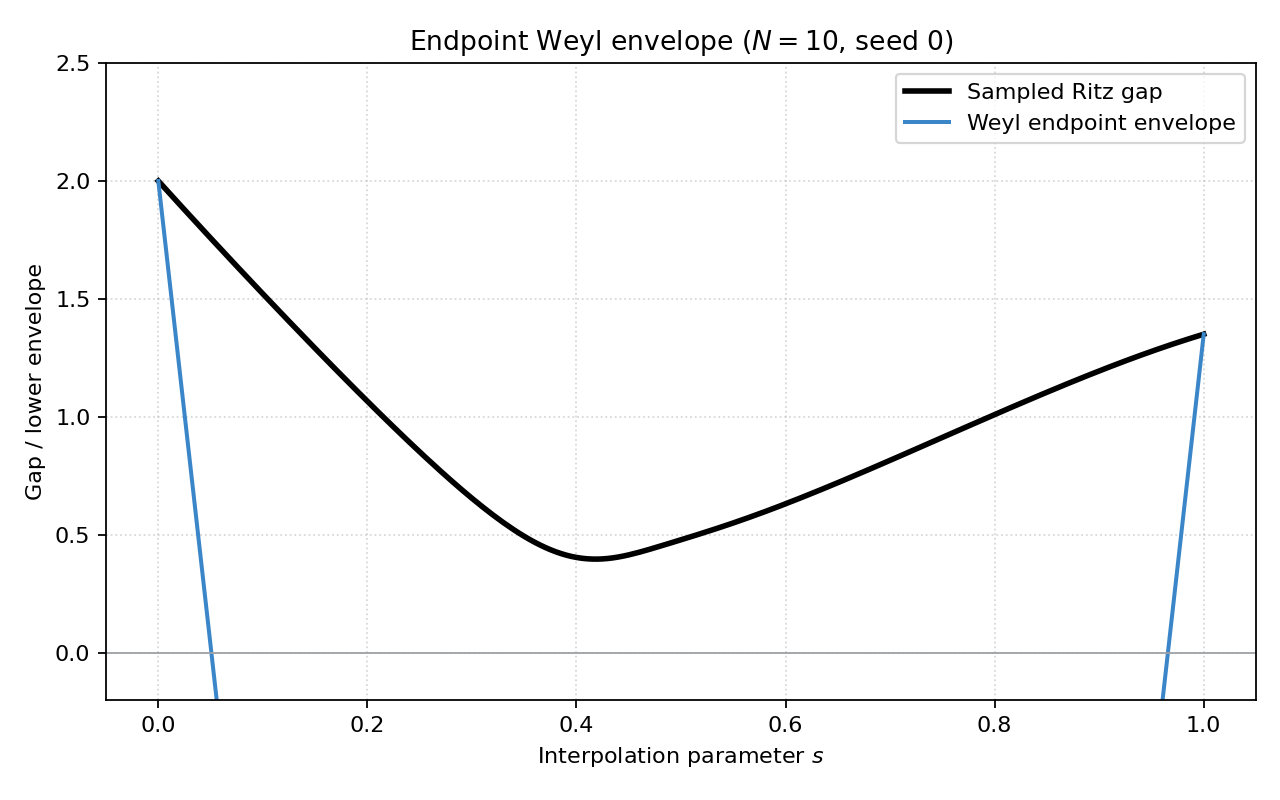
\includegraphics[width=0.88\textwidth]{comparison_updated_N10_no_anchors.png}
\caption{Conditional Weyl endpoint envelope for one connected weighted $N=10$ instance (seed $0$). The black curve samples the floating-point reduced-sector Ritz gap $\Delta_+$ and is not a verified continuous-path curve.}
\label{fig:no_anchors}
\end{figure}

Let
\begin{equation}
D_+:=H_{P,+}-H_{I,+},
\qquad
K_{\mathrm{gap},+}:=\lambda_{\max}(D_+)-\lambda_{\min}(D_+).
\end{equation}
A continuation input $K_{\mathrm{gap,cert}}$ must satisfy
\begin{equation}
0\le K_{\mathrm{gap},+}\le K_{\mathrm{gap,cert}},
\qquad
|\Delta_+(t)-\Delta_+(s)|\le K_{\mathrm{gap,cert}}|t-s|.
\end{equation}
The endpoint cones can be informative near the boundaries but are often too conservative in the middle of the path.

For the archived model, every stored binary64 edge weight is interpreted as an exact dyadic rational. Let
\begin{equation}
W_{\mathrm{exact}}:=\sum_{(i,j)\in E}w_{ij},
\qquad
\Lambda_I:=2\left\lfloor\frac{n_v}{2}\right\rfloor,
\end{equation}
where the sum is taken in exact rational arithmetic. Then
\begin{equation}
0\le H_{P,+}\le W_{\mathrm{exact}}I,
\qquad
0\le H_{I,+}\le\Lambda_I I,
\end{equation}
and therefore
\begin{equation}
-\Lambda_I I\le D_+\le W_{\mathrm{exact}}I,
\qquad
K_{\mathrm{gap},+}\le W_{\mathrm{exact}}+\Lambda_I.
\end{equation}
The implementation first forms the least binary64 number $W_{\mathrm{upper}}\ge W_{\mathrm{exact}}$ and then the least binary64 number not below the exact dyadic sum $W_{\mathrm{upper}}+\Lambda_I$. Thus
\begin{equation}
\label{eq:computational-gap-bounds}
\boxed{K_{\mathrm{gap,cert}}\ge W_{\mathrm{upper}}+\Lambda_I
\ge W_{\mathrm{exact}}+\Lambda_I\ge K_{\mathrm{gap},+}.}
\end{equation}
This is a direct spectral-width certificate with outward rounding. Table~\ref{tab:gap_diameter} compares its ensemble mean with ordinary floating-point estimates of the actual diameter $K_{\mathrm{gap},+}$.

\begin{table}[htbp]
\centering
\small
\begin{tabular}{cccc}
\toprule
$N$ & Estimated $K_{\mathrm{gap},+}$ & $K_{\mathrm{gap,cert}}$ & Cert./estimated \\
\midrule
\SectionSevenGapDiameterRows
\bottomrule
\end{tabular}
\caption{Means over 20 connected instances at each size. The diameter column is an ordinary floating-point extremal-eigenvalue diagnostic, whereas $K_{\mathrm{gap,cert}}$ is the outward-rounded analytic upper bound in Eq.~\eqref{eq:computational-gap-bounds}.}
\label{tab:gap_diameter}
\end{table}

The generated summary also reports how often the endpoint-only bounds are positive on the fixed diagnostic grid.
\begin{table}[htbp]
\centering
\small
\begin{tabular}{cccc}
\toprule
$N$ & Weyl endpoint & PSD floor (oracle) & PSD floor (poly.) \\
\midrule
\SectionSevenCoverageRows
\bottomrule
\end{tabular}
\caption{Mean sampled positive fractions over 20 instances at each size, evaluated on the 201-point diagnostic grid. The oracle PSD column uses full diagonal endpoint data; the polynomial-input column uses the spectral and greedy endpoint surrogates. These endpoint-only floating-point diagnostics are separate from the continuation interval classification.}
\label{tab:endpoint_coverage}
\end{table}

\subsection{Anchor Calculations and Certification Levels}
At each anchor $s_k$, SciPy's sparse Lanczos interface \texttt{eigsh} estimates the two lowest eigenpairs of $H_+(s_k)$. For reported Ritz pairs $(\theta_j,\ket{\psi_j})$, we monitor
\begin{equation}
r_j=\norm{\bigl(H_+(s_k)-\theta_jI\bigr)\ket{\psi_j}}_2,
\qquad j=0,1.
\end{equation}
For exact real-number inputs, the residual theorem gives
\begin{equation}
\operatorname{dist}\!\left(\theta_j,\operatorname{spec}H_+(s_k)\right)\le r_j.
\end{equation}
This existence statement does not identify the nearby eigenvalue's index or show that no lower eigenvalue was missed. Likewise, the exact Rayleigh quotient of a normalized trial vector upper-bounds $E_{0,+}(s_k)$, but the reported $\theta_0$ and $r_j$ are floating-point quantities without outward rounding. Treating those reported values as valid mathematical bounds, and conditional on $\theta_1$ representing the first excited eigenvalue, motivates the implemented anchor quantity
\begin{equation}
\label{eq:conditional-anchor}
\Delta_{+,\mathrm{lo}}(s_k)
:=\max\{0,(\theta_1-r_1)-\theta_0\}.
\end{equation}
The residual $r_0$ remains a convergence diagnostic but is not used in this formula. Equation~\eqref{eq:conditional-anchor} is therefore a conditional floating-point lower-bound estimate, not an independently verified indexed enclosure.

We distinguish three levels:
\begin{description}
\item[Level 1: formal implication.] Theorems apply to mathematical inputs satisfying their stated inequalities.
\item[Level 2: conditional floating-point continuation.] Sparse Ritz values and residual diagnostics supply routine sweep anchors without verified indexing or outward-rounded residual arithmetic.
\item[Level 3.] \textbf{Replayable exact indexed anchor.} Exact-dyadic Hamiltonian data and witness specifications are checked by an independent exact-arithmetic program that proves the indexed inequalities with no acceptance tolerance.
\end{description}
All continuous sweeps and aggregate continuation rows in this paper are Level~2. Only the four listed point anchors in the next subsection are Level~3; they do not constitute a Level-3 continuation.

\subsection{Representative Exact-Dyadic Level-3 Anchors}

Theorem~\ref{thm:exact-indexed-anchor} is applied to four seed-0 anchors. Archived binary64 edge weights, the binary64 parameter $s$, and both witness vectors are interpreted as exact dyadic rationals. SciPy is used only to propose a ground-state vector $q$, a strictly positive principal-submatrix witness $x$, a coordinate $p$, and a convenient $X$- or $Z$-basis representation; none of those floating-point proposals is trusted. The independent checker reconstructs the exact matrix, verifies $x>0$, evaluates $\ell$ and $U_0$ as rational numbers, and checks every scaled-diagonal-dominance inequality without an acceptance tolerance. A stored specification/result pair and the independent checker make each selected point verification replayable.

\begin{table}[htbp]
\centering
\small
\begin{tabular}{ccccc}
\toprule
$N$ & Seed & Binary64 input $s$ & Basis & Verified gap lower bound \\
\midrule
10 & 0 & $0.1$ & $X$ & $1.220109841289$ \\
10 & 0 & $0.4174116949186277$ & $Z$ & $0.159173111131$ \\
12 & 0 & $0.1$ & $X$ & $1.064501314437$ \\
12 & 0 & $0.5025125632610975$ & $Z$ & $0.067240247486$ \\
\bottomrule
\end{tabular}
\caption{Four selected replayable Level-3 anchors. The displayed bounds are decimal approximations to authoritative exact rational values $\ell-U_0>0$ stored in the verification records. These pointwise checks do not certify either continuous sweep.}
\label{tab:level3-anchors}
\end{table}

Figure~\ref{fig:with_anchors} shows how additional Level-2 anchors change the conditional envelope for one instance.
\begin{figure}[htbp]
\centering
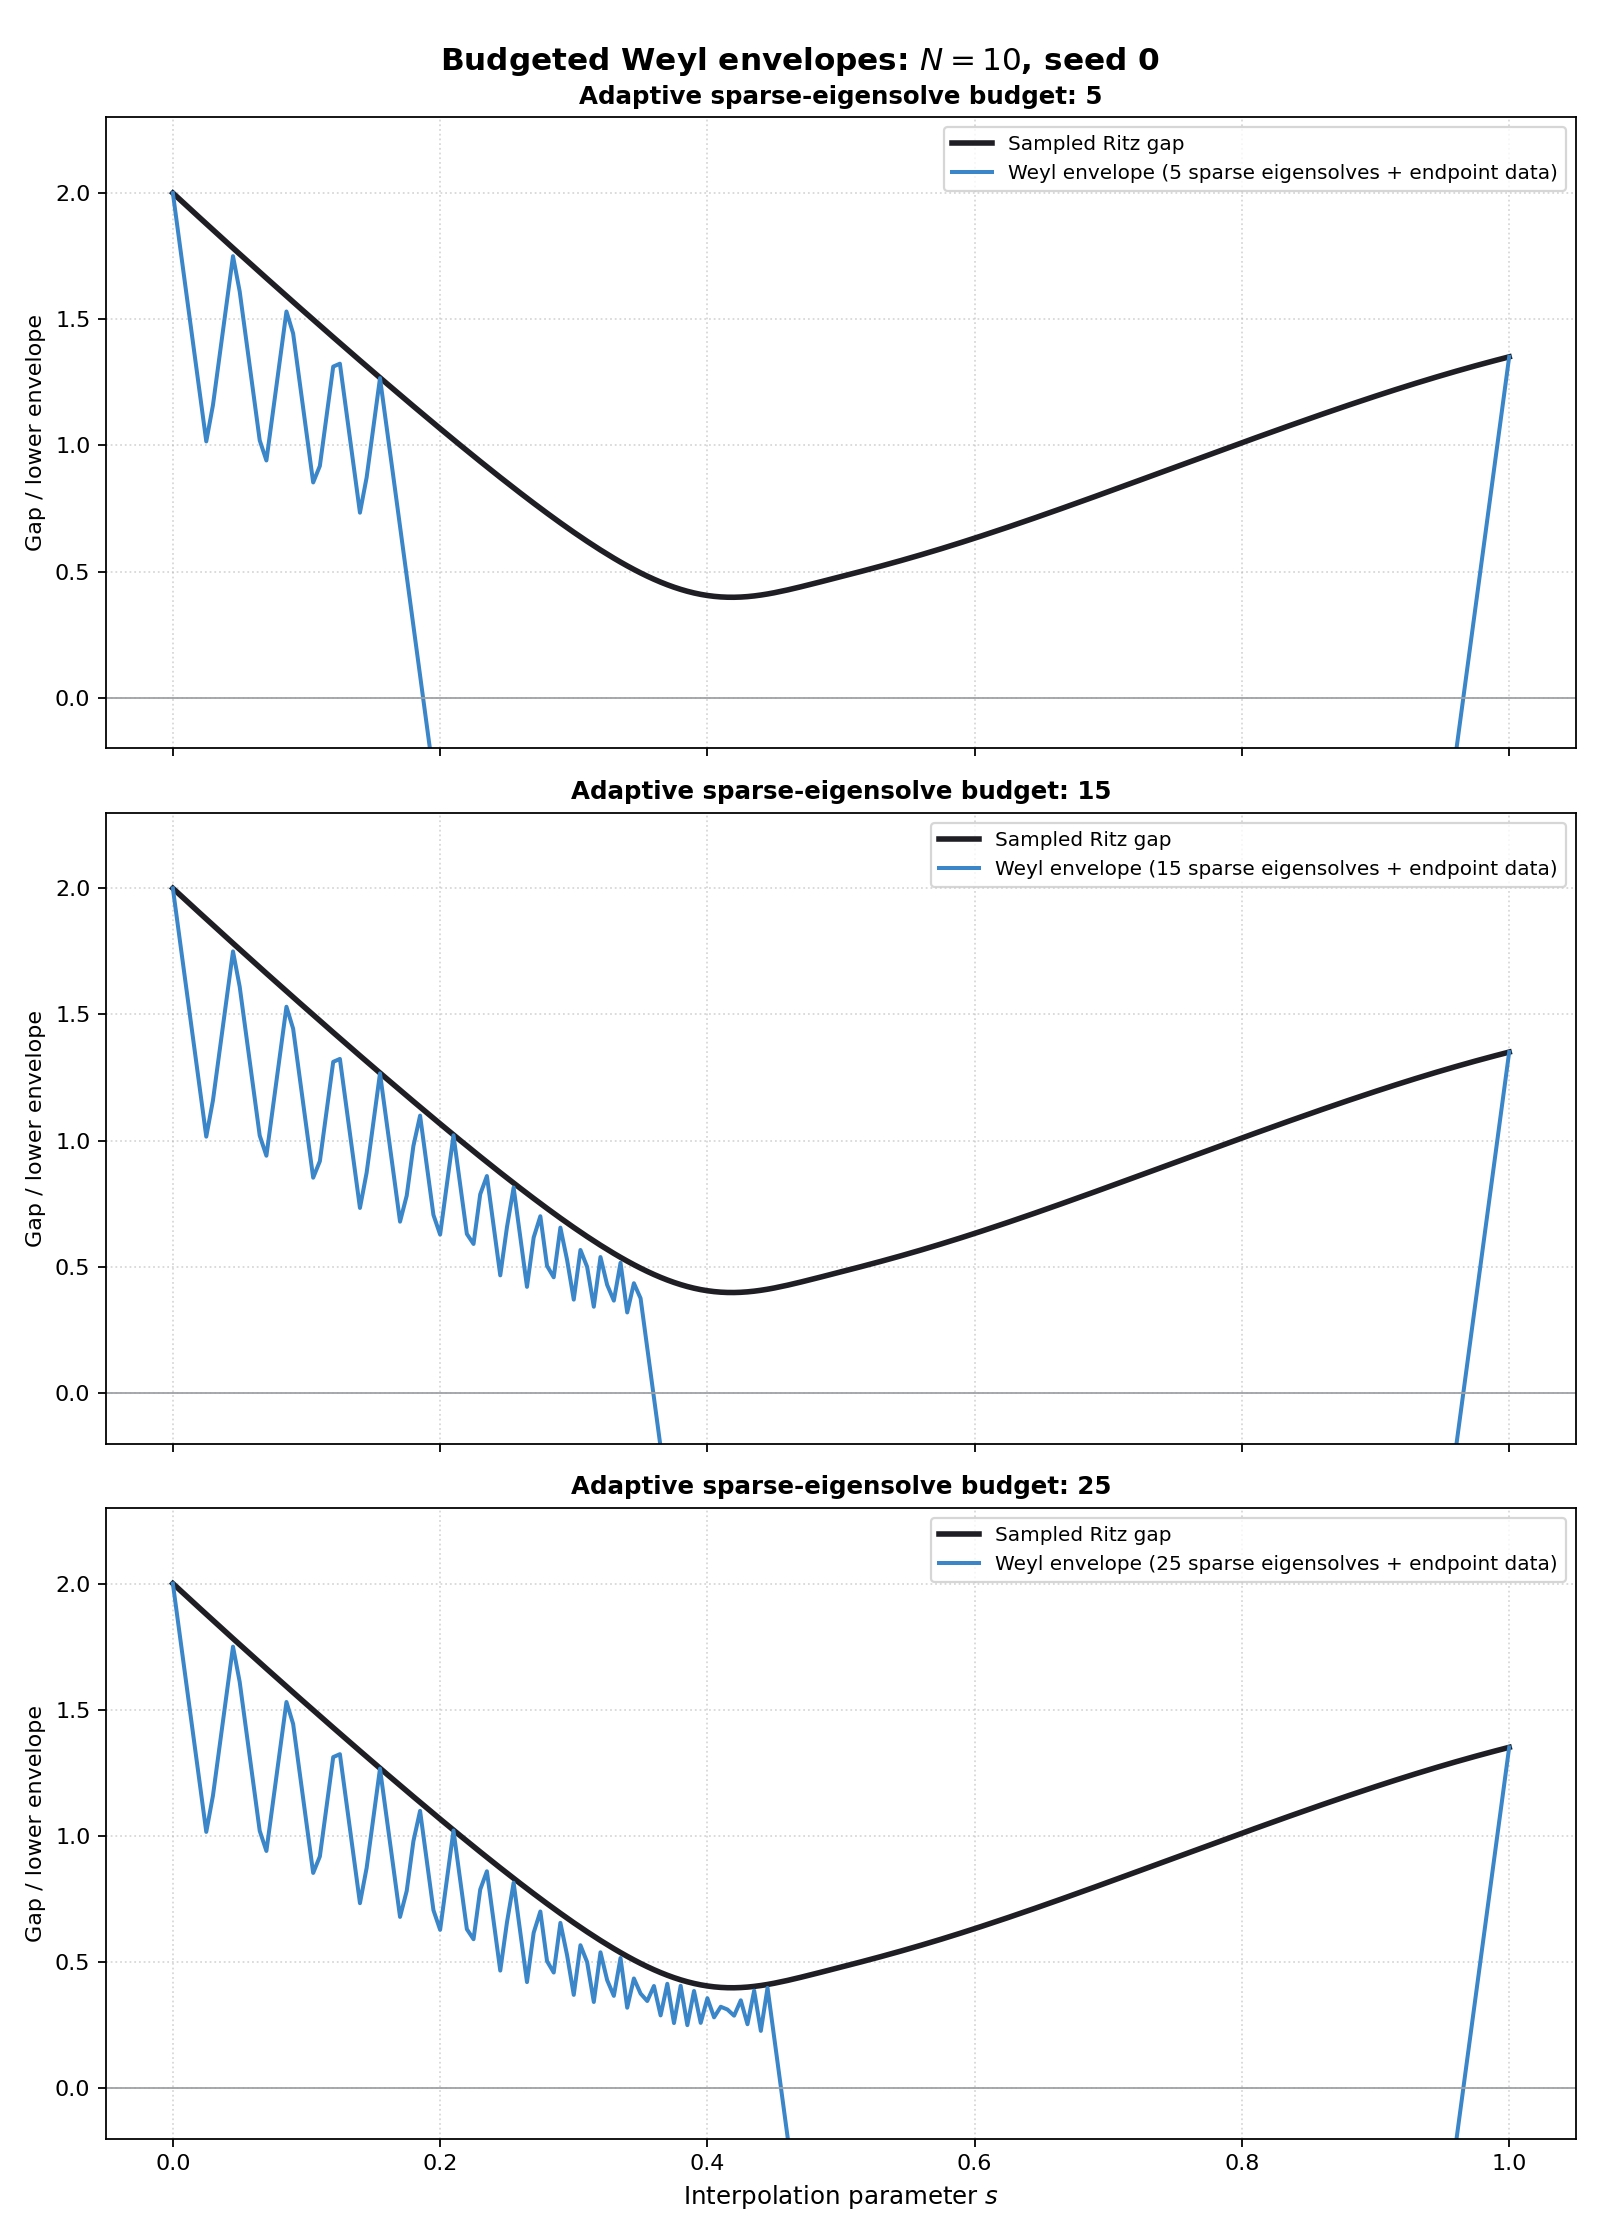
\includegraphics[width=0.88\textwidth]{comparison_updated_N10_anchors.png}
\caption{Budgeted conditional Weyl envelopes for one connected weighted $N=10$ instance (seed $0$). Each panel uses at most the stated number of sparse eigensolves plus endpoint information. The black curve is a sampled reduced-sector Ritz-gap reference $\Delta_+$; neither curve is a verified continuous-path enclosure.}
\label{fig:with_anchors}
\end{figure}

Each Level-2 anchor uses two Ritz values, residual diagnostics, and the supplied direct $K_{\mathrm{gap,cert}}$. Sparse Krylov methods avoid full dense diagonalization, but their cost depends on sparsity, tolerance, spectral separation, and warm-start quality; no linear-time eigensolve claim is made.

\subsection{Adaptive Continuation with Exponential Mark-and-Probe}
Let $\eta\in(0,1)$, $h_{\mathrm{floor}}>0$, and $K_{\mathrm{gap,cert}}\ge0$. For $K_{\mathrm{gap,cert}}>0$, the ordinary proposal at $s_k$ is
\begin{equation}
h_k^{\mathrm{prop}}:=\eta\frac{\Delta_{+,\mathrm{lo}}(s_k)}{K_{\mathrm{gap,cert}}},
\end{equation}
and the recorded floor-overridden length is
\begin{equation}
h_k^{\mathrm{floor}}:=\max\{h_k^{\mathrm{prop}},h_{\mathrm{floor}}\}.
\end{equation}
If $h_k^{\mathrm{prop}}<h_{\mathrm{floor}}$, the code marks a floor trigger and uses the probe-planned length
\begin{equation}
\label{eq:probe-plan}
h_k^{\mathrm{probe}}
:=\min\!\left\{\max(h_{\mathrm{floor}},0.05),
\max(h_{\mathrm{floor}},0.001)2^{q_k}\right\},
\end{equation}
where $q_k$ is the number of consecutive preceding floor triggers. An ordinary adaptive step instead uses $h_k^{\mathrm{probe}}=h_k^{\mathrm{floor}}=h_k^{\mathrm{prop}}$ and resets the trigger count to zero. In all modes, the actual endpoint-clipped length and its bound are
\begin{equation}
h_k^{\mathrm{act}}:=\min\{h_k^{\mathrm{probe}},1-s_k\},
\qquad
B_k:=\Delta_{+,\mathrm{lo}}(s_k)-K_{\mathrm{gap,cert}}h_k^{\mathrm{act}}.
\end{equation}
The actual interval is conditionally resolved if and only if $B_k>0$; a probe is not automatically unresolved merely because the floor triggered.

\begin{center}
\fbox{%
\begin{minipage}{0.94\linewidth}
\textbf{Algorithm 1: Adaptive continuation with mark-and-probe}

\smallskip
\textbf{Inputs:} $H_+(s)$; $K_{\mathrm{gap,cert}}\ge0$; $\eta\in(0,1)$; $h_{\mathrm{floor}}>0$; an anchor routine returning finite $\Delta_{+,\mathrm{lo}}(s)\ge0$.

\textbf{Outputs:} Anchors $\mathcal A$, interval records $\mathcal S$, and unresolved windows $\mathcal U$.

\begin{enumerate}[label=\arabic*., leftmargin=2em, itemsep=0.3em, topsep=0.4em]
    \item Initialize $s\leftarrow0$, $q\leftarrow0$, and $\mathcal A,\mathcal S,\mathcal U\leftarrow\emptyset$.
    \item \textbf{While} $s<1$:
    \begin{enumerate}[label=\alph*., leftmargin=1.8em, itemsep=0.2em, topsep=0.2em]
        \item Obtain $\delta\leftarrow\Delta_{+,\mathrm{lo}}(s)$ and add $(s,\delta)$ to $\mathcal A$.
        \item \textbf{If} $K_{\mathrm{gap,cert}}=0$, set
        $h^{\mathrm{prop}}=h^{\mathrm{floor}}=h^{\mathrm{probe}}\leftarrow1-s$
        and $q\leftarrow0$.
        \item \textbf{Otherwise}, set $h^{\mathrm{prop}}\leftarrow\eta\delta/K_{\mathrm{gap,cert}}$ and $h^{\mathrm{floor}}\leftarrow\max\{h^{\mathrm{prop}},h_{\mathrm{floor}}\}$.
        If $h^{\mathrm{prop}}<h_{\mathrm{floor}}$, mark a floor trigger and set
        \begin{equation*}
        h^{\mathrm{probe}}\leftarrow
        \min\{\max(h_{\mathrm{floor}},0.05),
        \max(h_{\mathrm{floor}},0.001)2^q\},
        \qquad q\leftarrow q+1.
        \end{equation*}
        Otherwise use the normal adaptive step $h^{\mathrm{probe}}\leftarrow h^{\mathrm{prop}}$ and set $q\leftarrow0$.
        \item Apply the endpoint clip $h^{\mathrm{act}}\leftarrow\min\{h^{\mathrm{probe}},1-s\}$ and calculate $B\leftarrow\delta-K_{\mathrm{gap,cert}}h^{\mathrm{act}}$.
        \item Classify $[s,s+h^{\mathrm{act}}]$ as conditionally resolved iff $B>0$; otherwise add it to $\mathcal U$. Record the proposed, floor-overridden, probe-planned, and actual lengths and the classification fields in $\mathcal S$, then update $s\leftarrow s+h^{\mathrm{act}}$.
    \end{enumerate}
    \item \textbf{Return} $\mathcal A$, $\mathcal S$, and the merged windows $\mathcal U$.
\end{enumerate}
\end{minipage}%
}
\end{center}

A valid $K_{\mathrm{gap,cert}}=0$ means that $D_+$ is scalar and $\Delta_+$ is constant. The explicit branch therefore advances to the endpoint without division and classifies the interval from $B_k=\Delta_{+,\mathrm{lo}}(s_k)$.

\begin{theorem}[Conditional Positivity from the Actual Step]
\label{thm:continuation-positivity}
Assume $0\le K_{\mathrm{gap},+}\le K_{\mathrm{gap,cert}}$ and that an interval starts from a valid anchor bound
\begin{equation}
0\le\Delta_{+,\mathrm{lo}}(s_k)\le\Delta_+(s_k).
\end{equation}
Then, for every $s\in[s_k,s_{k+1}]$,
\begin{equation}
\label{eq:actual-step-bound}
\Delta_+(s)\ge B_k
=\Delta_{+,\mathrm{lo}}(s_k)-K_{\mathrm{gap,cert}}h_k^{\mathrm{act}}.
\end{equation}
Consequently, the classification accepts exactly intervals with $B_k>0$, and every accepted interval is conditionally positive. If $K_{\mathrm{gap,cert}}>0$ and the step is an ordinary adaptive step, then
\begin{equation}
B_k\ge(1-\eta)\Delta_{+,\mathrm{lo}}(s_k).
\end{equation}
For an accepted floor-triggered probe, positivity follows directly from $B_k>0$; no $(1-\eta)\Delta_{+,\mathrm{lo}}(s_k)$ bound is asserted. If $K_{\mathrm{gap,cert}}=0$, then $B_k=\Delta_{+,\mathrm{lo}}(s_k)$.
\end{theorem}

\begin{proof}
Theorem~\ref{thm:lipschitz-gap} gives
\begin{equation}
\Delta_+(s)\ge\Delta_{+,\mathrm{lo}}(s_k)
-K_{\mathrm{gap,cert}}(s-s_k)
\ge\Delta_{+,\mathrm{lo}}(s_k)
-K_{\mathrm{gap,cert}}h_k^{\mathrm{act}}=B_k.
\end{equation}
The classification implication is immediate. For an ordinary adaptive step, endpoint clipping gives
\begin{equation}
h_k^{\mathrm{act}}\le h_k^{\mathrm{prop}}
=\eta\Delta_{+,\mathrm{lo}}(s_k)/K_{\mathrm{gap,cert}},
\end{equation}
which yields the stated safety-factor bound. A probe can be longer than $h_k^{\mathrm{prop}}$, so only its explicitly computed $B_k$ is used. The zero-constant case follows by substitution.
\end{proof}

\begin{theorem}[Termination and Interval-Count Bounds]
\label{thm:termination}
Under the algorithmic hypotheses above, and provided every requested anchor call returns a finite nonnegative quantity, Algorithm~1 terminates regardless of whether those quantities are valid gap lower bounds. Unconditionally,
\begin{equation}
\label{eq:unconditional-termination}
N_{\mathrm{int}}\le\left\lceil\frac{1}{h_{\mathrm{floor}}}\right\rceil.
\end{equation}
If, in addition, every returned anchor quantity satisfies $\Delta_{+,\mathrm{lo}}(s_k)\ge\delta_{\mathrm{lo}}>0$, then the refined bound is
\begin{equation}
\label{eq:refined-termination}
N_{\mathrm{int}}\le
\begin{cases}
\displaystyle
\left\lceil
\frac{1}{\max\{h_{\mathrm{floor}},\eta\delta_{\mathrm{lo}}/K_{\mathrm{gap,cert}}\}}
\right\rceil,&K_{\mathrm{gap,cert}}>0,\\[1.2ex]
1,&K_{\mathrm{gap,cert}}=0.
\end{cases}
\end{equation}
\end{theorem}
\begin{proof}
For $K_{\mathrm{gap,cert}}>0$, an ordinary probe-planned length is at least $h_{\mathrm{floor}}$, while Eq.~\eqref{eq:probe-plan} makes a floor-triggered probe at least $\max\{h_{\mathrm{floor}},0.001\}\ge h_{\mathrm{floor}}$. Every non-final actual step equals its probe-planned length; only the final step can be shortened by endpoint clipping. This proves Eq.~\eqref{eq:unconditional-termination}. If all returned anchor quantities are at least $\delta_{\mathrm{lo}}$, every ordinary proposal is at least $\eta\delta_{\mathrm{lo}}/K_{\mathrm{gap,cert}}$, and a floor-triggered probe occurs only when that proposal is below $h_{\mathrm{floor}}$. Hence every non-final step is at least $\max\{h_{\mathrm{floor}},\eta\delta_{\mathrm{lo}}/K_{\mathrm{gap,cert}}\}$, proving Eq.~\eqref{eq:refined-termination}. If $K_{\mathrm{gap,cert}}=0$, the explicit branch advances directly to $s=1$ in one interval.
\end{proof}
Here $N_{\mathrm{int}}$ counts accepted and unresolved intervals. With one anchor solve at the start of each interval, the recorded solve count equals $N_{\mathrm{int}}$; an independent terminal-endpoint solve would add one. The refined termination hypothesis concerns returned quantities only and does not assert that they are valid lower bounds on $\Delta_+$.

\subsection{Schema-4 Conditional Records and Exact Anchor Records}
For an interval starting at $s_k$, the schema-4 conditional log records
\begin{equation}
\mathcal C_k=\bigl(s_k,s_{k+1},\delta_k,K_{\mathrm{gap,cert}},
 h_k^{\mathrm{prop}},h_k^{\mathrm{floor}},h_k^{\mathrm{probe}},
 h_k^{\mathrm{act}},f_k^{\mathrm{floor}},f_k^{\mathrm{clip}},m_k,B_k,\rho_k\bigr),
\end{equation}
where the four length entries correspond to \texttt{h\_proposed}, \texttt{h\_floor\_overridden}, \texttt{h\_probe\_planned}, and \texttt{h\_actual}; $f_k^{\mathrm{floor}}$ and $f_k^{\mathrm{clip}}$ are the floor-trigger and endpoint-clip flags; $m_k$ identifies adaptive, floor-mark-and-probe, or constant-gap mode; and $\rho_k$ contains the Boolean resolution status and reason. Thus $h_k^{\mathrm{floor}}$ is the simple floor override, $h_k^{\mathrm{probe}}$ is the planned pre-clip probe, and $h_k^{\mathrm{act}}$ is the traversed length. The defining checks are
\begin{equation}
h_k^{\mathrm{act}}=\min\{h_k^{\mathrm{probe}},1-s_k\}
=s_{k+1}-s_k,
\qquad
B_k=\delta_k-K_{\mathrm{gap,cert}}h_k^{\mathrm{act}},
\qquad
\rho_k=\mathrm{resolved}\Longleftrightarrow B_k>0.
\end{equation}
For a floor trigger, a verifier reconstructs the consecutive-trigger exponent $q_k$ from the preceding flags and checks Eq.~\eqref{eq:probe-plan}, the probe cap, and endpoint clipping. For an ordinary step it checks $h_k^{\mathrm{floor}}=h_k^{\mathrm{probe}}=h_k^{\mathrm{prop}}$. These algebraic checks prove propagation only if the anchor inequality $\delta_k\le\Delta_+(s_k)$ is valid.

Each Level-2 log has schema version \SectionSevenResultSchema{} and stores the exact numerator and denominator of $W_{\mathrm{exact}}$, $W_{\mathrm{upper}}$, and $K_{\mathrm{gap,cert}}$, together with the direct derivation in Eq.~\eqref{eq:computational-gap-bounds}; Ritz values and residuals; solver and probe policies; complete interval records; graph hashes; and provenance. The Level-2 logs do not verify their own eigenvalue indices. The four Level-3 anchor specifications and results are separate replayable records containing exact hashes, exact rational $U_0$, $\ell$, and $\ell-U_0$, and all no-tolerance comparison checks. Their scope statements explicitly leave the continuous sweeps at Level~2.

\begin{figure}[htbp] \centering 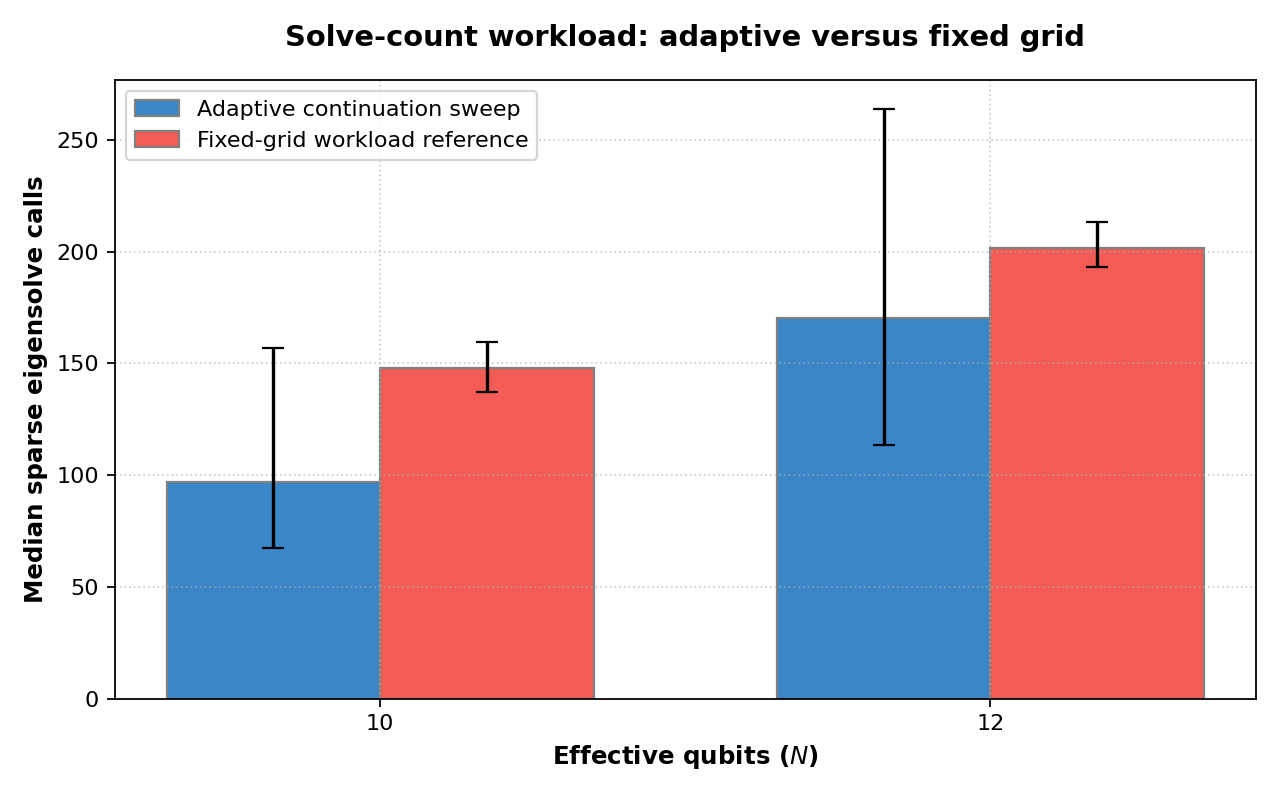
\includegraphics[width=\textwidth]{efficiency_comparison.png} \caption{Sparse-eigensolve counts for the adaptive continuation sweep and a fixed-grid workload reference, over 20 connected instances at each displayed size (seeds 0--19). Bars show medians and error bars show interquartile ranges. The methods do not provide matched guarantees, so the figure reports workload rather than speedup.} \label{fig:efficiency} \end{figure}

\begin{figure}[htbp] \centering 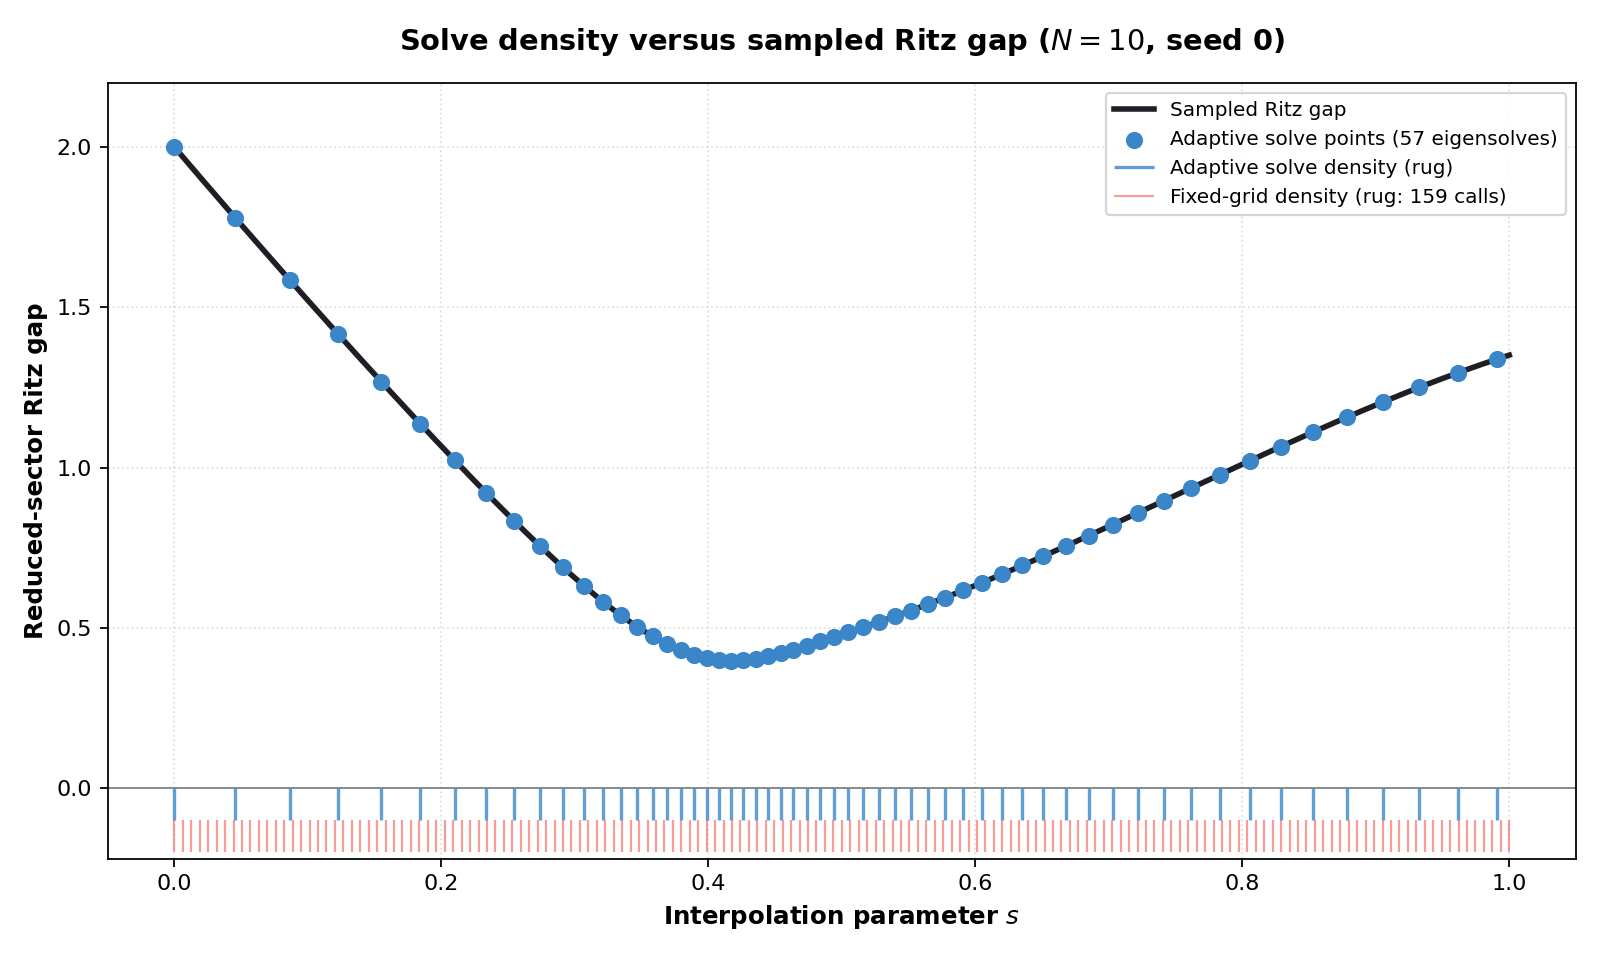
\includegraphics[width=\textwidth]{grid_density_vs_gap.png} \caption{Adaptive and fixed-grid solve locations relative to a sampled floating-point reduced-sector Ritz-gap curve $\Delta_+$ for the connected $N=10$, seed-0 instance. The plot visualizes placement only; it is not a verified gap plot.} \label{fig:grid_N10} \end{figure}

Figures~\ref{fig:grid_N10} and \ref{fig:grid_N12} visualize the solve locations for the seed-0 instances. In these examples, adaptive locations are denser in portions of the sampled curve with smaller Ritz gaps. Each location still requires a sparse eigensolve, whose cost depends on convergence as well as call count.

\begin{figure}[htbp]
\centering
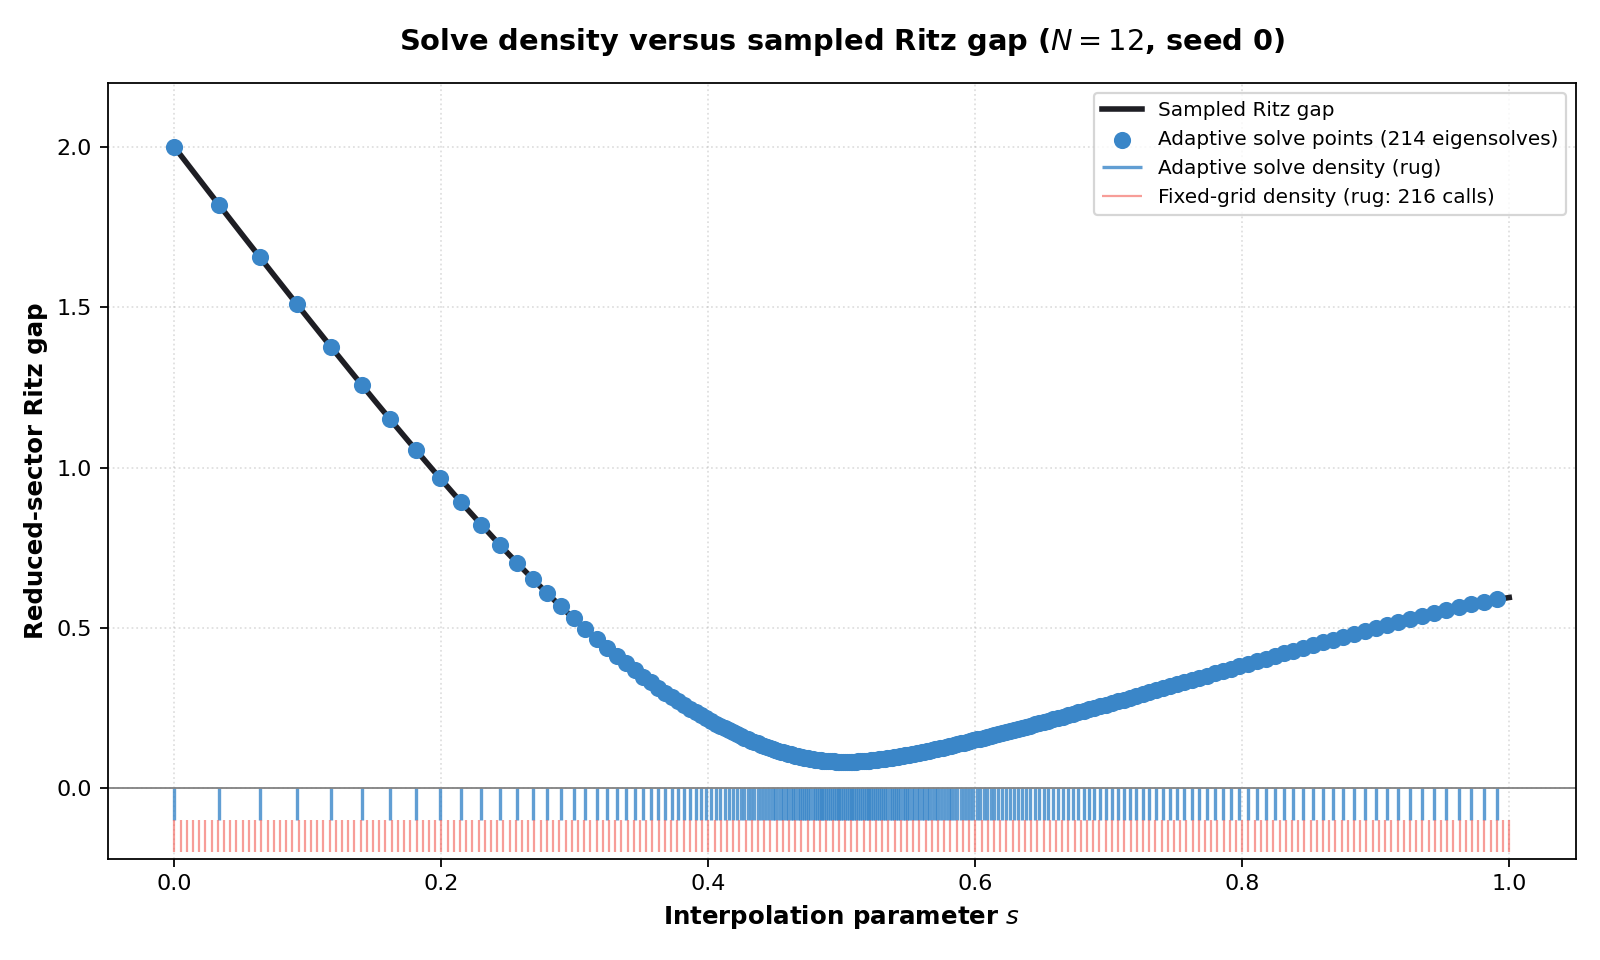
\includegraphics[width=\textwidth]{grid_density_vs_gap_N12.png}
\caption{Adaptive and fixed-grid solve locations relative to a sampled floating-point reduced-sector Ritz-gap curve $\Delta_+$ for the connected $N=12$, seed-0 instance.}
\label{fig:grid_N12}
\end{figure}


The adaptive and fixed-grid constructions distribute evaluations differently. In the regenerated sample, the adaptive call count can be smaller or larger than the selected fixed-grid workload; narrow sampled gaps can lead to many adaptive calls.

\subsubsection{Experimental Specification and Setup}
We assess the lower-bound output and workload of Algorithm~1 under the following setup:
\begin{itemize}
    \item \textbf{Graph generation:} Weighted Erd\H{o}s--R\'{e}nyi graphs $G(n_v,p=0.5)$ have $n_v=N+1$ physical vertices, so $\dim\mathcal H_+=2^N$. Edge weights are independent draws from $[0.5,1.5]$.
    \item \textbf{Instance filtering:} Instances are resampled until the graph is connected and a floating-point reduced-sector calculation reports a nondegenerate problem ground state. As an independent artifact check, exact dyadic enumeration confirms endpoint nondegeneracy for all 40 retained graphs.
    \item \textbf{Eigensolvers and parameters:} Level-2 anchors and spectral-diameter diagnostics use \texttt{eigsh} with tolerance $10^{-10}$; anchors use $k=2$, \texttt{which='SA'}, \texttt{ncv}$=\min(d_+,50)$, SciPy's default maximum-iteration policy, a deterministic initial vector, and the previous ground-state Ritz vector as the next warm start. An ARPACK nonconvergence exception terminates the affected run. The sweep uses $\eta=0.9$, $h_{\mathrm{floor}}=10^{-6}$, the direct outward-rounded $K_{\mathrm{gap,cert}}$ from Eq.~\eqref{eq:computational-gap-bounds}, and mark-and-probe scales $10^{-3}$ and $0.05$. The auxiliary fixed-grid workload uses $\delta_{\mathrm{ref}}=0.25$.
    \item \textbf{Hardware and software:} The implementation uses Python 3.12.10 and was run on a standard desktop computer with a 12th Gen Intel(R) Core(TM) i5-1245U and 16 GB of RAM. Eigensolve wall-clock times are a secondary performance metric.
\end{itemize}

\subsubsection{Performance Statistics}
The following tables import their rows from \texttt{results/section7\_summary.tex}, generated from \SectionSevenInstanceCount{} validated schema-\SectionSevenResultSchema{} instance rows.

\begin{table}[htbp]
\centering
\small
\setlength{\tabcolsep}{5pt}
\begin{tabular}{ccccccc}
\toprule
$N$ & \multicolumn{2}{c}{Sparse-eigensolve calls} & \multicolumn{4}{c}{Relative count change (\%)} \\
\cmidrule(r){2-3} \cmidrule(r){4-7}
& Uniform Grid & Adaptive Sweep & Mean $\pm$ SD & Min & Median & Max \\
\midrule
\SectionSevenSolveCountRows
\bottomrule
\end{tabular}
\caption{Solve-count workload over 20 instances at each size. Counts are median / mean $\pm$ population SD. Negative relative changes mean that mark-and-probe continuation used more calls. The uniform grid uses $h_{\mathrm{uniform}}=\delta_{\mathrm{ref}}/K_{\mathrm{gap,cert}}$ as a workload reference, not a matched-certification baseline.}
\label{tab:anchor_stats}
\end{table}

For a complete sweep, define its reported global conditional lower bound as the nonnegative part of $\min_k B_k$. It is strictly positive exactly when every interval is conditionally resolved. Table~\ref{tab:global-conditional} includes zero for an unresolved sweep when forming the ensemble mean.
\begin{table}[htbp]
\centering
\small
\begin{tabular}{ccccc}
\toprule
$N$ & Globally resolved & Mean lower bound & Minimum & Maximum \\
\midrule
\SectionSevenGlobalConditionalRows
\bottomrule
\end{tabular}
\caption{Global Level-2 conditional gap lower bounds. For $N=12$, the ensemble mean includes the unresolved run with reported value zero. These quantities remain conditional on the sparse-anchor indexing assumptions.}
\label{tab:global-conditional}
\end{table}

\begin{table}[htbp]
\centering
\small
\begin{tabular}{ccccc}
\toprule
$N$ & Continuation-resolved & Mean windows & Mean width & Maximum width \\
\midrule
\SectionSevenUnresolvedRows
\bottomrule
\end{tabular}
\caption{Merged unresolved-window statistics. The sole unresolved $N=12$ sweep contains one width-$0.001$ mark-and-probe window; it is not a sequence of hundreds of microscopic floor steps. ``Continuation-resolved'' refers only to the Level-2 interval classification.}
\label{tab:unresolved_stats}
\end{table}

The $N=12$ call-count distribution is skewed by the two largest runs: 2153 adaptive calls for seed 9 and 1439 for seed 13. The seed-13 run contains the sole unresolved mark-and-probe interval, of width $0.001$. These are observed workloads, not complexity bounds. Exponential probes reduce redundant floor-region solves while retaining the full unresolved mark whenever the actual-length bound is nonpositive.

The data show instance-dependent workload rather than a uniform speedup. The sampled $\Delta_+$ curves are visual diagnostics, and the global values in Table~\ref{tab:global-conditional} quantify the reach of the conditional continuation bounds. Table~\ref{tab:gap_diameter} shows the conservatism of the direct outward-rounded $K_{\mathrm{gap,cert}}$ relative to floating-point diameter estimates. Anchor count alone does not determine wall-clock cost because Krylov convergence and warm-start quality also vary.

\subsection{Integral-Based Cost Model}
Ignoring endpoint clipping, floor overrides, and integer rounding, the implemented rule suggests the continuum approximation
\begin{equation}
\label{eq:integral_cost}
N_{\mathrm{heuristic}}\approx\frac{K_{\mathrm{gap,cert}}}{\eta}
\int_0^1\frac{\dd s}{\widetilde\Delta_{+,\mathrm{lo}}(s)}.
\end{equation}
The implementation does not evaluate this expression from an interpolated anchor-bound curve. For the selected diagnostic run only, it substitutes a sampled floating-point Ritz-gap curve:
\begin{equation}
N_{\mathrm{heuristic}}\approx\frac{K_{\mathrm{gap,cert}}}{\eta}
\int_0^1\frac{\dd s}{\Delta_+(s)}.
\end{equation}
This is an idealized cost interpretation, not a complexity bound. It omits anchor error, floor overrides, endpoint clipping, and integer effects. Moreover, prediction and observation are not statistically independent if both are generated from the same reference gap and step rule.

The regenerated data contain a computed integral only for the diagnostic $N=10$, seed-0 run: the sampled-reference trapezoidal estimate gives $56.52$, versus 57 adaptive solves. No ensemble integral analysis is reported. The single close match is illustrative rather than a validation of the model.

\section{Future Research}

Several extensions would make the framework more useful.
\begin{enumerate}
    \item \textbf{Non-affine paths.} For
    \begin{equation}
    H(s)=a(s)H_I+b(s)H_P+c(s)H_C,
    \end{equation}
    a local certificate should use the spectral width of the relevant path increment or derivative, not its uncentered norm. Such an extension must account for varying coefficients and cannot infer catalyst effectiveness from PSD monotonicity alone.

    \item \textbf{Class-specific structure.} Other graph ensembles, 3-SAT, and Subset Sum may have symmetries or positivity properties that establish nonclosing independently of continuation. Future experiments should separate such structural results from the quantitative question of how tight propagated lower bounds are.

    \item \textbf{Verified and quantum-assisted anchors.} The four replayable exact-dyadic checks demonstrate Level~3 verification at selected points. Extending Level~3 to a full continuation would require independently verified indexed anchors at every requested location, for example through verified inertia or interval eigensolvers coupled to the same interval records. At larger $N$, phase estimation or quantum subspace/Krylov methods \cite{Parrish2019, Stair2020} might supply anchor information, but state-preparation cost, statistical uncertainty, and eigenvalue indexing would all need explicit validation.
\end{enumerate}

\section{Conclusions}

For an affine Hermitian path with $D=H_P-H_I$, the relevant Weyl constant for the first gap is the shift-invariant spectral width
\begin{equation}
K_{\mathrm{gap}}=\lambda_{\max}(D)-\lambda_{\min}(D)
=2\min_{c\in\mathbb R}\norm{D-cI}_2,
\end{equation}
not, in general, the larger comparison value $2\norm{D}_2$. Using a valid upper bound $K_{\mathrm{gap,cert}}$, the continuation theorem propagates valid anchor lower bounds over intervals classified by $B_k>0$. The schema-4 bookkeeping distinguishes proposed, floor-overridden, probe-planned, and actual endpoint-clipped lengths, treats $K_{\mathrm{gap,cert}}=0$ explicitly, and gives both an unconditional termination bound and a refined bound.

The regenerated sparse Max-Cut sweeps remain conditional Level-2 floating-point assessments: all 20 $N=10$ runs and 19 of 20 $N=12$ runs are conditionally resolved, with one width-$0.001$ unresolved interval for $N=12$, seed 13. Perron--Frobenius irreducibility gives interior ground-state uniqueness for these reduced stoquastic paths, while exact dyadic enumeration independently confirms endpoint nondegeneracy for all 40 archived graphs. Accordingly, the aggregate continuation results quantify lower-bound conservatism and workload rather than establish a previously unknown positivity property or a speedup. PSD monotonicity supplies only componentwise energy comparisons and has no standalone gap-amplification implication.

Four selected seed-0 anchors do have replayable Level-3 exact-dyadic records: an independent no-tolerance checker proves indexed lower bounds by comparison matrices, interlacing, and exact Rayleigh quotients. These pointwise certificates do not make either continuation Level~3. A full Level-3 sweep would require independently checkable indexed enclosures at every continuation anchor. The present contribution remains a transparent assembly of classical inequalities and auditable bookkeeping, not a new matrix inequality or a verified many-body gap computation.

\section{Accessibility of the Code and Data}

The code and data are publicly available at \url{https://github.com/TiagoVerissimo/Bounding_Spectral_Gaps}. The repository includes the schema-4 continuation records and generated \path{results/section7_summary.tex}, together with the selected Level-3 exact-dyadic specifications, exact result records, and independent checker. Hashes and exact rational payloads make the four point anchors replayable; the accompanying scope metadata keeps the continuous sweeps at Level~2.


\bibliographystyle{plain}
\bibliography{references}

\end{document}
